% SIAM Shared Information Template
% This is information that is shared between the main document and any
% supplement. If no supplement is required, then this information can
% be included directly in the main document.
Keeping in mind the observations from previous \cref{Sec:motivation}, one could observe that it would be best to maintain the non-zeros of matrix close to the diagonal. This has been observed previously in the regard of normal sparse matrix computations %TODO cite
 like \SpMV and has led to the pre-processing of matrix by applying bandwidth reduction algorithms like ``\RCMfull" (\RCM). Now we aim to develop a method that does not distort this ideal permutations to a large extent but at the same time resolve \DK dependencies. 
 
Our approach can be seen as a recursive level based method. Each step of the method basically consists of four steps namely:
\begin{enumerate}
	\item Level construction
	\item Permutation
	\item Distance-k coloring
	\item Load balancing
\end{enumerate}
The method is strongly coupled to the hardware underneath and exploits only the parallelism as required by the hardware. If at the end of all these four steps one does not achieve sufficient parallelism, all the steps are recursively applied to selected sub-graphs of the matrix until sufficient parallelism is attained. This recursive nature of our coloring method led to the naming of the method as ``\RACEfull" in short \RACE.

To explain the method in an easier and illustrative way we choose a simple matrix namely the 2D 7\pt stencil. The sparsity pattern and the corresponding graph of the matrix is as shown in \cref{fig:2d-7pt}.

\begin{figure}[tbhp]
	\centering
	\subfloat[Sparsity
	 pattern]{\label{fig:2d-7pt-a}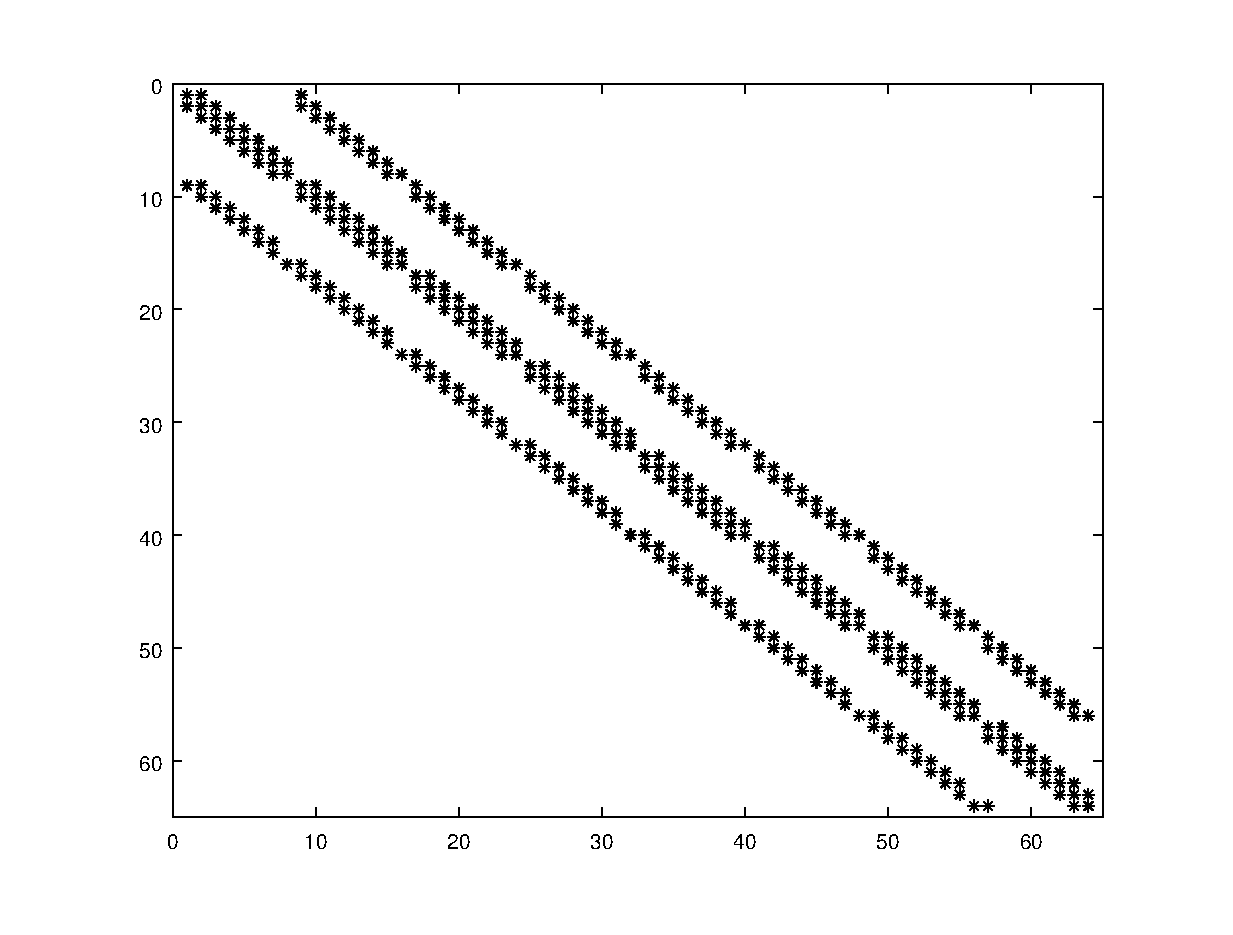
\includegraphics[width=0.4\textwidth , height=0.2\textheight]{pics/2d-7pt/2d_7pt_bw.eps}}
	\hspace{1.5em}
	\subfloat[Graph]{\label{fig:2d-7pt-b}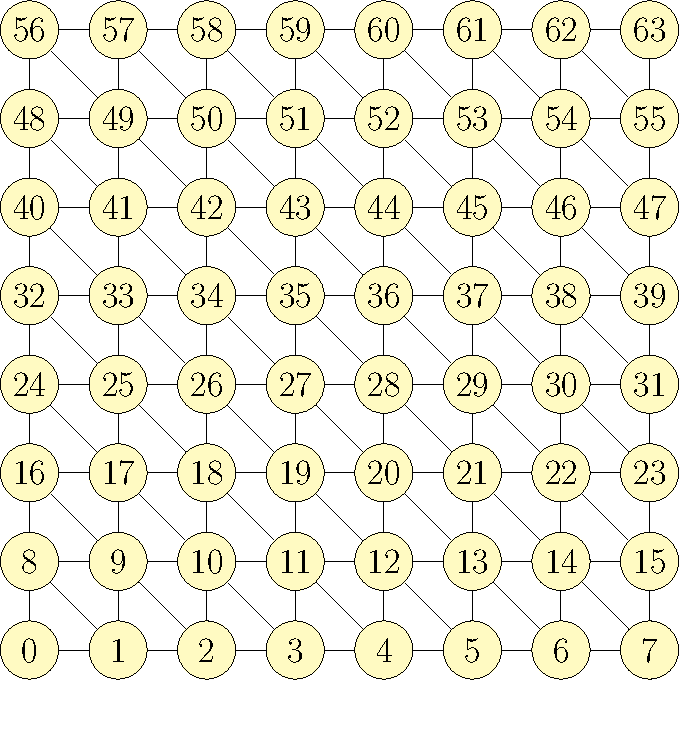
\includegraphics[width=0.35\textwidth , height=0.19\textheight]{pics/2d-7pt/stencil_2d_7pt.pdf}}
	\caption{2d-7pt Stencil}
	\label{fig:2d-7pt}
\end{figure}

\subsection*{Definitions}
The following basic definitions from graph theory are used in the following sections:
\begin{itemize}
	\item \textbf{Graph : } $G = (V,E)$ represents a graph where $V(G)$ belongs to set of vertices and $E(G)$ represents the edges in the graph. Note that here we specifically denote $G$ for irreducible undirected graphs.
	\item \textbf{Neighborhood :} Neighborhood of vertex $u$ represented as $N(u)$ is defined as:
	\begin{equation*}
	  N(u) = \set{ v : uv \in E}
	\end{equation*}
	\item \textbf{Subgraph :} A subgraph $H$ of graph $G$ in this paper specifically refers to subgraph induced by $V' \subseteq V(G)$ and is defined as
	\begin{equation*}
		H = (V', \set{ uv : uv \in E(G) \text{ and } u,v \in V'})
	\end{equation*}
\end{itemize}

\subsection{Level Construction}\label{subsec:LEVEL_CONST}
The first step of the \RACE method is level construction. The step concerns with finding different \levels in the graph, \levels used here are same to the ones found in ``Breadth First Search" (\BFS) algorithm \cite{BFS}. First \level ($L(0)$) is chosen to consist of a selected root vertex. Rest of the levels ($L(i)$ for $i > 0$) are defined to  contain vertices that are in neighborhood of vertices in previous \level ($L(i-1)$) and not in $L(i-2)$ \cite{BFS_level_def} \ie
\begin{equation}\label{eq:level}
L(i) = 
\begin{cases}
	  u : u \in N(L(i-1)) \cap \overline{N(L(i-2))}  & \text{ if } i \neq 0 \\
	 root & otherwise
\end{cases}   
\end{equation}

 One could easily observe from \cref{eq:level} $i$-th \level consist of all vertices that have a minimum distance of $i$ from the root node. \Cref{alg:BFS} shows an algorithm to find each nodes minimum distance from root. Total number of levels obtained with this graph traversal will be denoted as \totalLvl. \Cref{fig:2d_7pt_level_construction} shows \levels on the \STEX (\totalLvl = 14), the main number on each vertex (v) refers to the vertex number and the superscript shows the \level number, \ie
\begin{equation}\label{eq:node_notation}
	v^i \implies v \in L(i)
\end{equation}
Note that this is substantially different to the \levels in methods like ``level-scheduling" \cite{saad} where depth (maximum distance) is sought after.

\begin{figure}[tbhp]
	\centering
	\subfloat[Level construction]{\label{fig:2d_7pt_level_construction}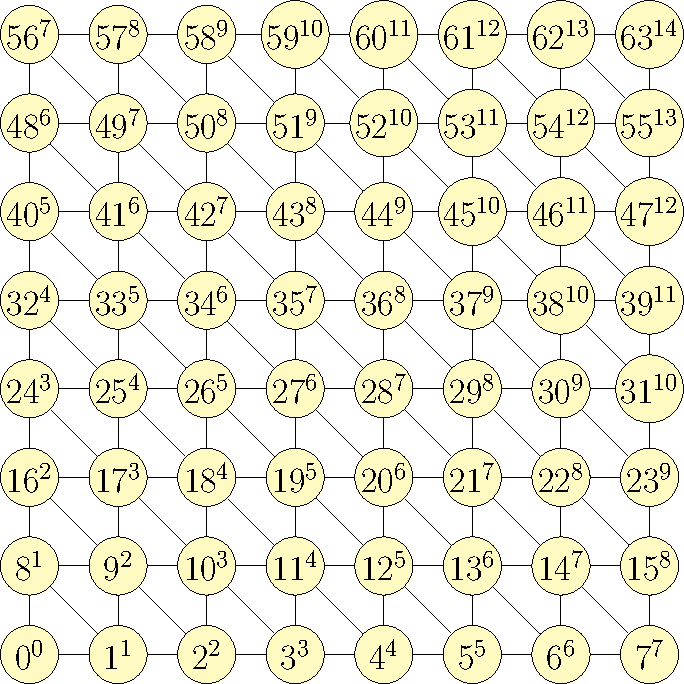
\includegraphics[height=0.18\textheight,width=0.32\textwidth]{pics/level_construction/stencil_2d_7pt}}
	\hspace{1em}
	\subfloat[Permuted graph ($G'$)]{\label{fig:2d_7pt_perm}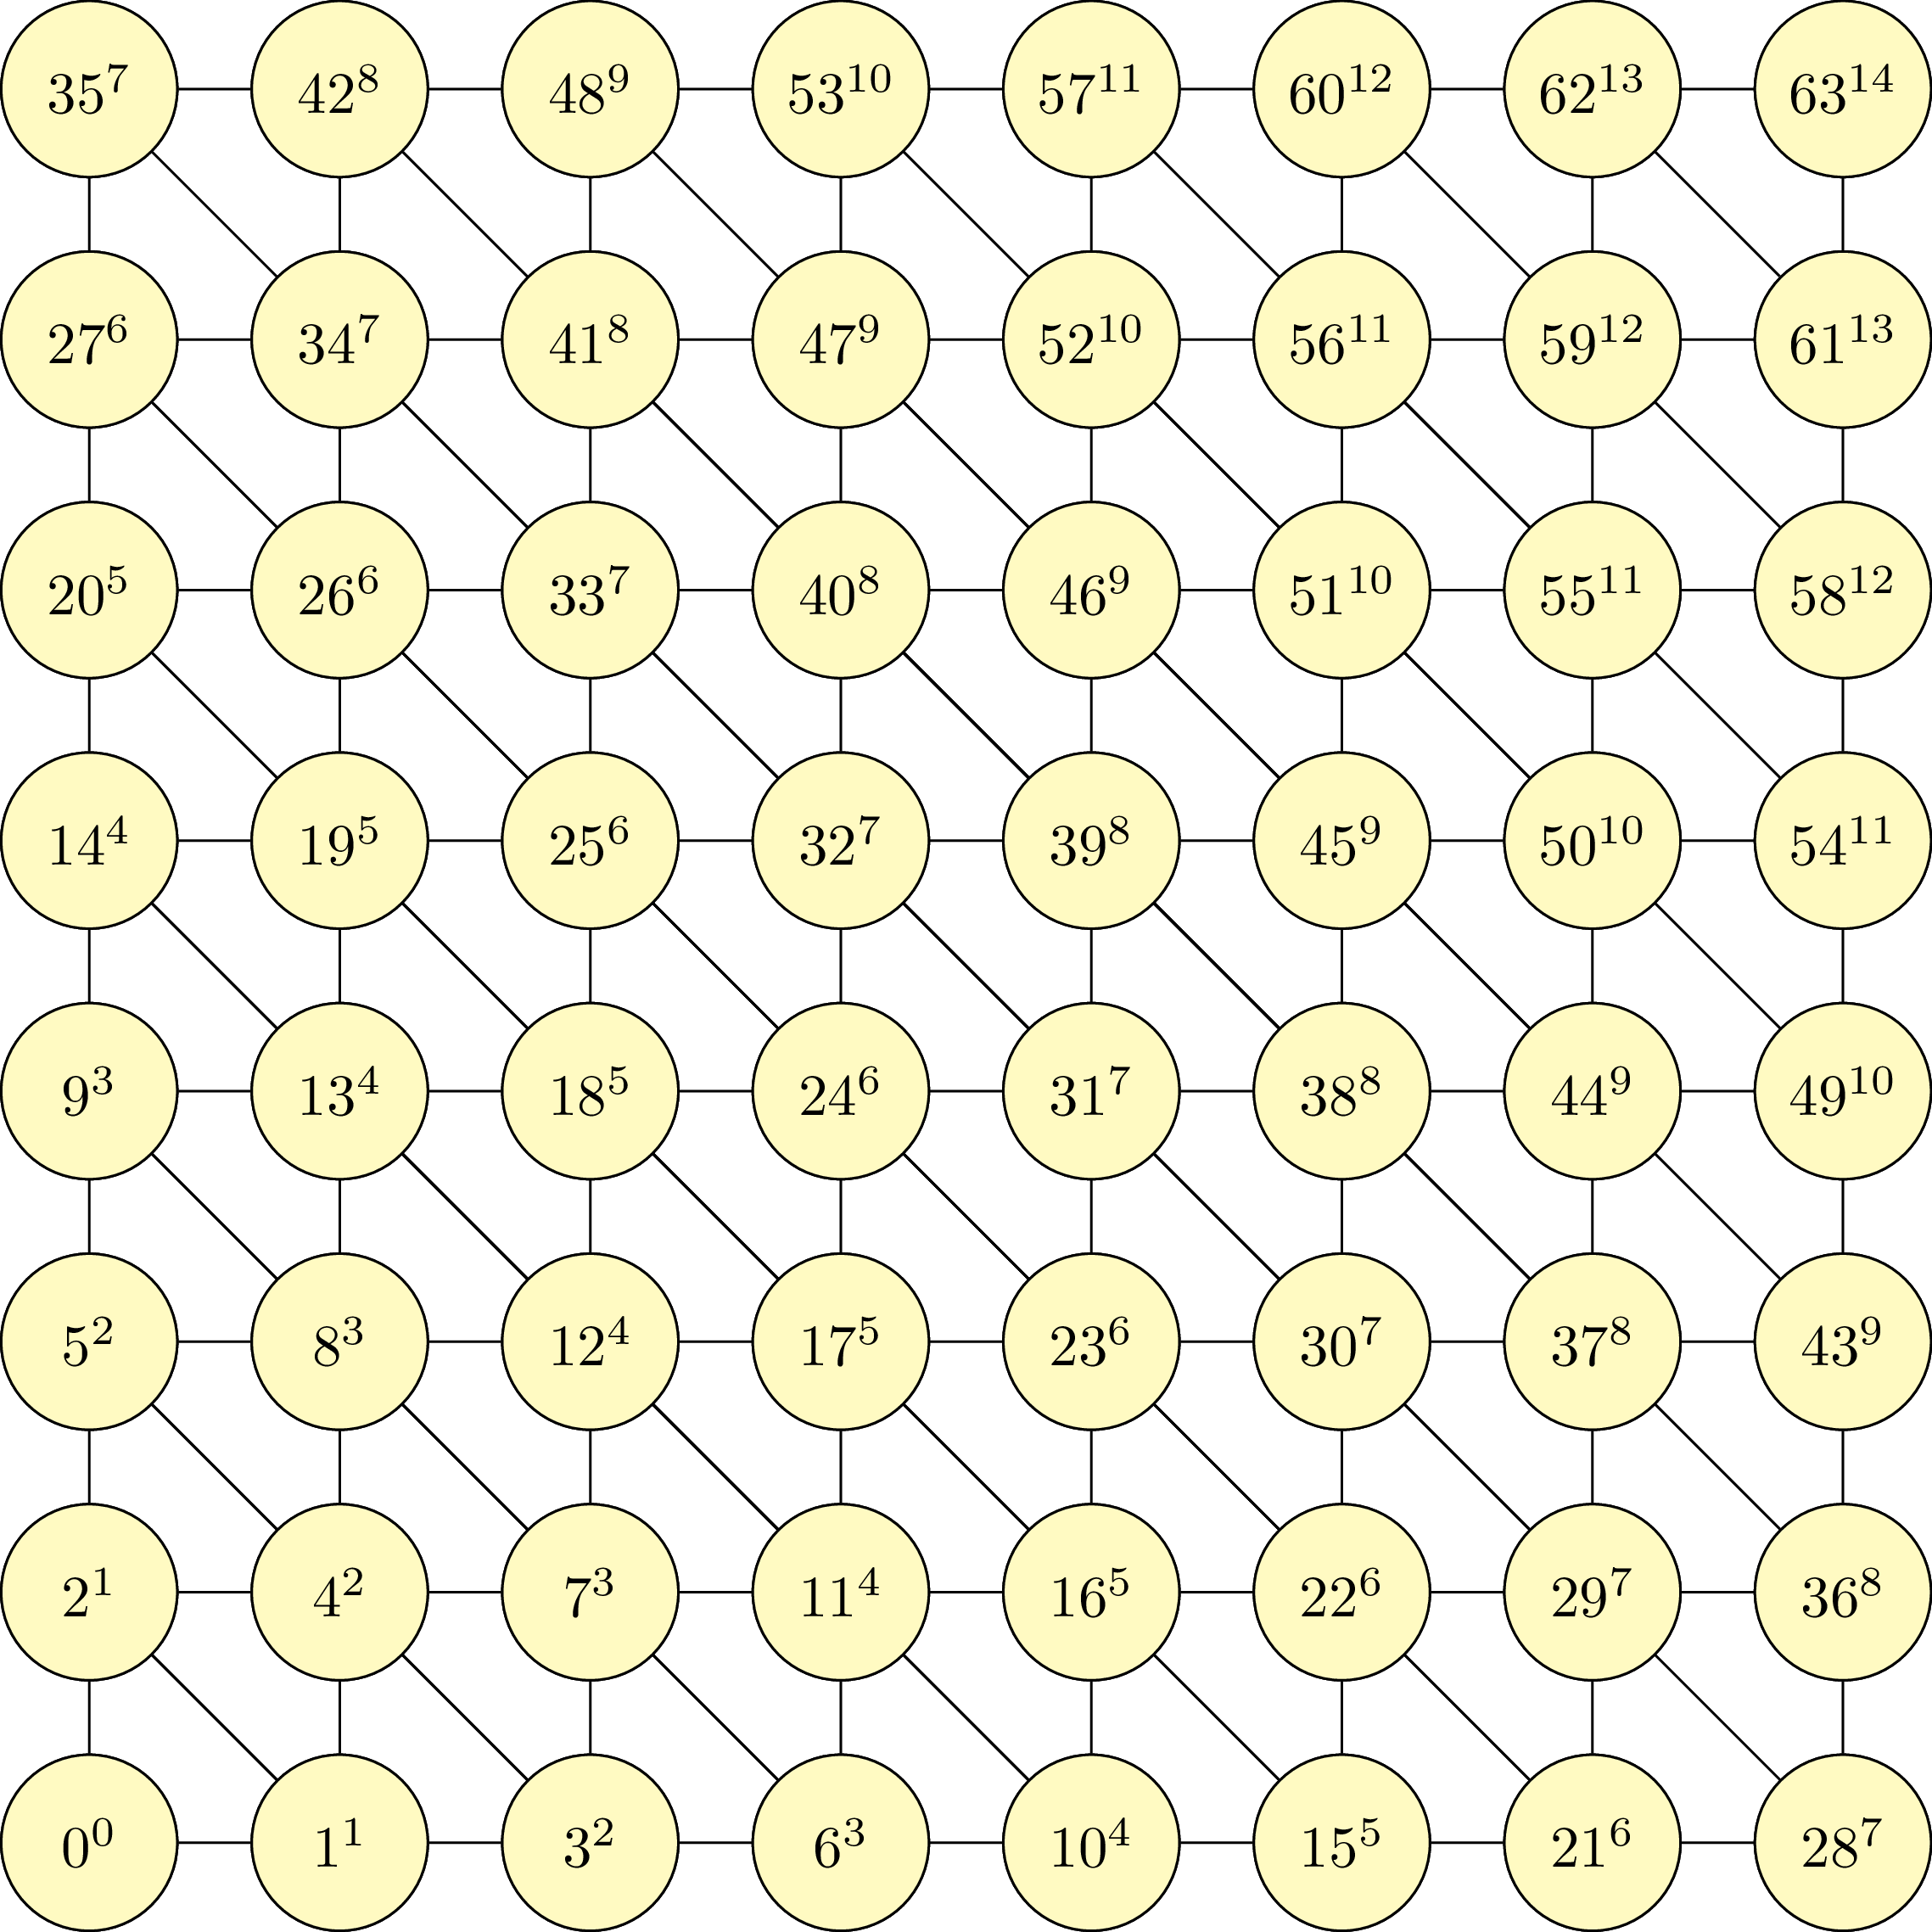
\includegraphics[height=0.18\textheight,width=0.32\textwidth]{pics/permutation/stencil_2d_7pt}}
	\hspace{1em}
	\subfloat[]{\label{fig:2d_7pt_levelPtr}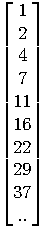
\includegraphics[height=0.18\textheight,width=0.07\textwidth]{pics/permutation/levelPtr}}
	\caption{(a) Levels in \STEX, (b) shows graph $G'$ after permutation and (c) is the associated \levelPtr to $G'$.}
	\label{fig:2d-7pt_step_1_2}
\end{figure}


\subsection{Permutation}\label{subsec:PERM}
Once the \levels are known one has to permute the matrix in the order of its \levels, such that vertices in $L(i)$ appears before that of $L(i-1)$. Till this step the procedure is similar to that of \BFS pre-processing for bandwidth reduction. One could also replace \BFS with better bandwidth reduction algorithms like ``(Reverse) \CMfull". \Cref{fig:2d-7pt_step_1_2} shows the graph ($G' = P(G)$) of \STEX matrix after this permutation ($P$) is applied. Observe the difference in node numbering between original lexicographic ordering in \cref{fig:2d_7pt_level_construction} and \cref{fig:2d_7pt_perm}. Now the most important step for resolving dependencies (coloring) is to store the information about \levels. \Inorder to do this we use a data structure called \levelPtr. It stores the starting vector of each \levels, which implies that \levels on $G'$ can be identified as:
\begin{equation*}
	L(i) = \set{ u : u \in [\levelPtr[i]:(\levelPtr[i+1]-1)] \text{ and } u \in V(G')}
\end{equation*}

 \levelPtr for \STEX example is shown in \cref{fig:2d_7pt_levelPtr}, and one could easily read from \levelPtr that vertices from $\levelPtr(4)=7$ to $\levelPtr(5)-1=10$ belongs to $L(4)$.
 
 
 \subsection{Distance-k coloring} \label{subsec:DK}
 Two vertices are called \DK neighbours if the shortest path connecting them consists of at most $k$ edges \cite{dist_k_def}. This implies $u$ is a \DK neighbour of $v$ (denoted as $u\xrightarrow{k}v$)  if
 \begin{equation}\label{eq:dk}
	  u\xrightarrow{k}v  \iff  v \in \set{ u \cup N(u) \cup N^2(u) \cup ... N^k(u) }	 
 \end{equation}
 Since we consider only undirected graph $u\xrightarrow{k}v$ also implies $v\xrightarrow{k}u$. 
  After having the permuted graph $G'$ one can show that $L(i)$ and $L(i+k+j)$ where $j\geq1$ are \DK independent as shown in the following \cref{corollary_dk}:
  \begin{corollary}\label{corollary_dk}
   $L(i)$ and $L(i\pm(k+j))$ are \DK independent $\forall j\geq1$. 
  \end{corollary}
  \begin{proof}
  	We prove by contradiction. Let there exist $u,v \in V(G')$ such that  $u \in L(i)$ and $v \in  L(i \pm (k+j) \forall j\geq1$. Assume $u,v$ are \DK neighbours ($u\xrightarrow{k}v$). From \cref{eq:level}, \cref{eq:dk} and the fact $G'$ is undirected we get 
  	\begin{align*}
	  	u\xrightarrow{k}v \iff & v \in \set{L(i) \cup L(i \pm 1) \cup ... \cup L(i \pm k)} \\
	  	\implies & v \notin L(i \pm (k+j) \text{  } \forall j \geq 1
  	\end{align*}
  	which is a contradiction to the fact $v \in L(i \pm (k+j) ) \forall j \geq 1$, this implies $u$ and $v$ are \DK independent.
  \end{proof}

\Cref{corollary_dk} implies that if we leave a gap of \emph{\atleast} one \level between any two \levels ($L(i), L(i+2)$ for example) all the vertices between them are \DONE independent. Similarly if there is a gap of \emph{\atleast} two \levels between any two \levels ($L(i), L(i+3)$ for example) we get \DTWO independent levels.
  
 \begin{figure}[tbhp]
 	\centering
 	\subfloat[\DONE independent \levelGroups]{\label{fig:2d_7pt_d1}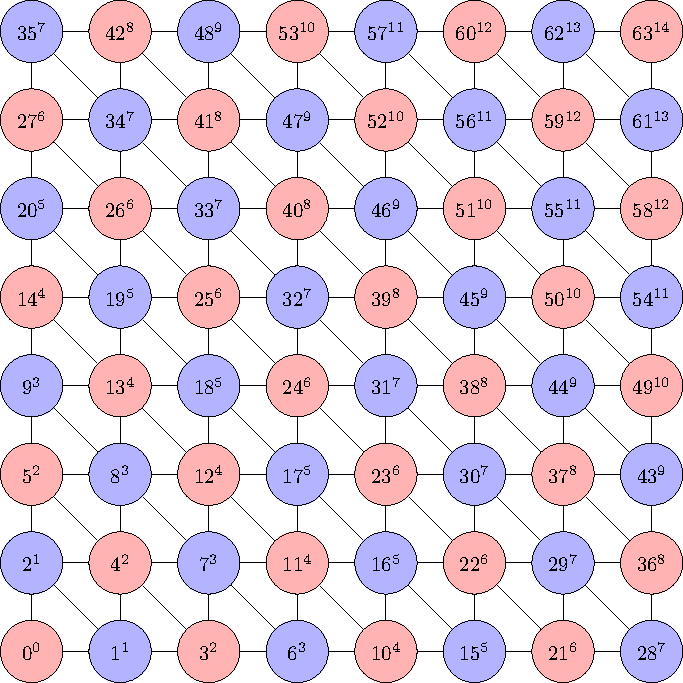
\includegraphics[height=0.2\textheight,width=0.4\textwidth]{pics/dk_coloring/stencil_2d_7pt_d1}}
 	\hspace{2.5em}
 	\subfloat[\DTWO independent \levelGroups]{\label{fig:2d_7pt_d2}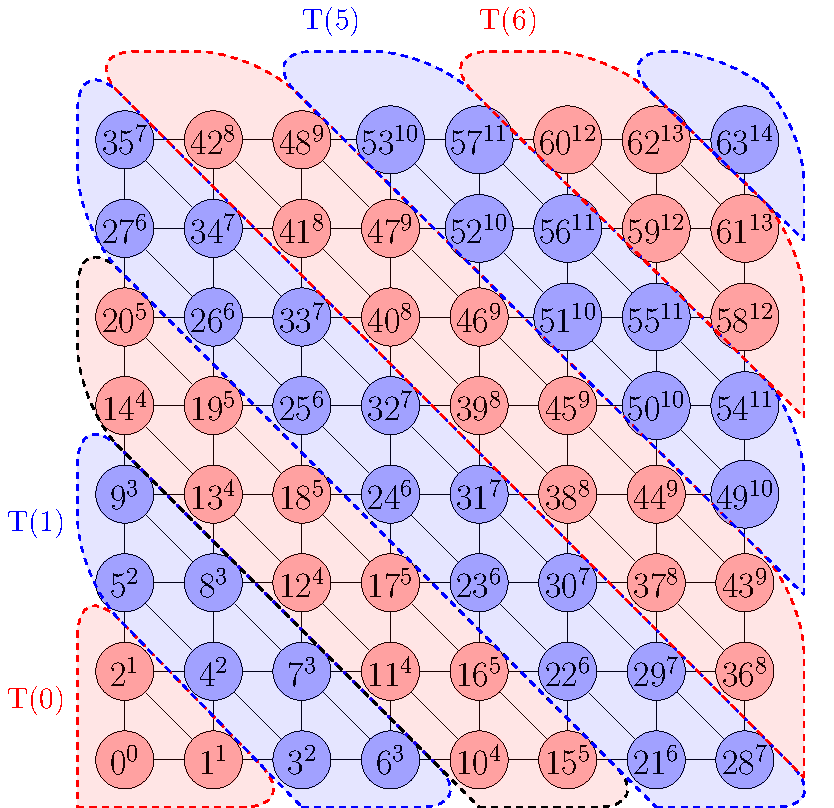
\includegraphics[height=0.23\textheight,width=0.48\textwidth]{pics/dk_coloring/stencil_2d_7pt_d2_with_lg}}
 	\caption{\DONE and \DTWO independent \levelGroups.}
 	\label{fig:2d-7pt_d1_d2}
 \end{figure}
 
  Due to this weak definition in \cref{corollary_dk} there exists many possibility to make \levels independent of each other and \cref{fig:2d-7pt_d1_d2} shows one such possibility each for \DONE and \DTWO independent \levels. One could group some of the nearby \levels together to form a \levelGroup, and make this \DONE or \DTWO independent of other \levelGroups. The $i$-th \levelGroup would be denoted by $T(i)$. Difference between \level and  \levelGroup can be seen in \cref{fig:2d_7pt_d2}, for \cref{fig:2d_7pt_d1} \levelGroup and \level coincides.
  
  In principle one could compute on all independent \levelGroups in parallel, but sequentially within a \levelGroup, i.e. for example in \cref{fig:2d_7pt_d2} $T(0)$, $T(2)$, $T(4)$, $T(6)$ can be operated by four different threads in parallel and in the next sweep rest \levelGroups. For the configurations seen in \cref{fig:2d-7pt_d1_d2} this would mean we have $\frac{\totalLvlMATH}{2}$ and $\frac{\totalLvlMATH}{4}$ parallelism for \DONE and \DTWO kernels respectively.
  
  But the problem with the configurations like the one seen in \cref{fig:2d-7pt_d1_d2} is that there is load imbalances between threads as the number of rows (\nrows) per \levelGroup is not distributed evenly. As seen here in the case of \STEX the threads working on extreme ends of graph (\eg $T(1), T(7)$) have small amount of work compared to the threads working on middle (\eg $T(3), T(4)$). 
  
  \subsection{Load balancing}\label{subsec:LB}
  Depending on the matrix each \levelGroup would contain different number of rows, which leads to load imbalances as seen above in \cref{subsec:DK}. \Inorder to avoid this problem we employ a load balancing scheme. At this step we plug in detail from hardware side like total parallelism. The idea is to exploit only the parallelism as required by the hardware while at the same time maintain \DK constraint seen in \cref{corollary_dk}. To balance the load more nearby \levels would be added to a \levelGroup which has less number of \nrows and at \levelGroup where we have considerably big \levels only sufficient amount of \levels to maintain \DK constraint would be assigned. Assigning nearby levels instead of a random level further helps in preserving data locality. 
  
  An algorithm for load balancing can be found in \cref{alg:LB}. The aim of the algorithm is to reduce combined variance of number of rows ($\nrowsMath(T(i))$) in each \levelGroup $T(i)$. It does this by calculating mean and variance of $T\_size$ in each parallel sweeps, where $T\_size(i)=\nrowsMath(T(i))$. For example in \cref{fig:2d_7pt_d2} we need to calculate mean of $T\_size$ of all \levelGroups in red sweep and blue sweep separately. The combined variance is then found by summing up the variances in each parallel sweep. \Inorder to reduce this combined variance we select the \levelGroup that has biggest absolute deviation from mean and try to add/remove levels to/from this \levelGroup from/to a \levelGroup that has biggest/least signed deviation. While removing \levels from a \levelGroup one has to take care that the \DK coloring is not violated, for example in case of \DTWO and two sweep scheme as seen in \cref{fig:2d_7pt_d2} we need to ensure at least two levels remain in a \levelGroup. To aid this shifting of \levels to/from \levelGroup we use the pointers to \levelGroup denoted by $T\_ptr$. Doing this process in an iterative way finally we end up in a state with lowest combined variance at which no further moves are possible either due to violation of \DK dependency or due to increase in combined variance. \Cref{fig:lb_alg} shows step by step procedure involved in load balancing and \cref{fig:2d_7pt_lb} shows \levelGroups after load balancing applied on \STEX example of size $16 \times 16.$

  One could also do this entire load balancing based on number of non-zeros (\nnz) rather than \nrows, in this case $T\_size(i)=\nnzMath(T(i))$.
  
   \begin{figure}[tbhp]
   	\centering
   	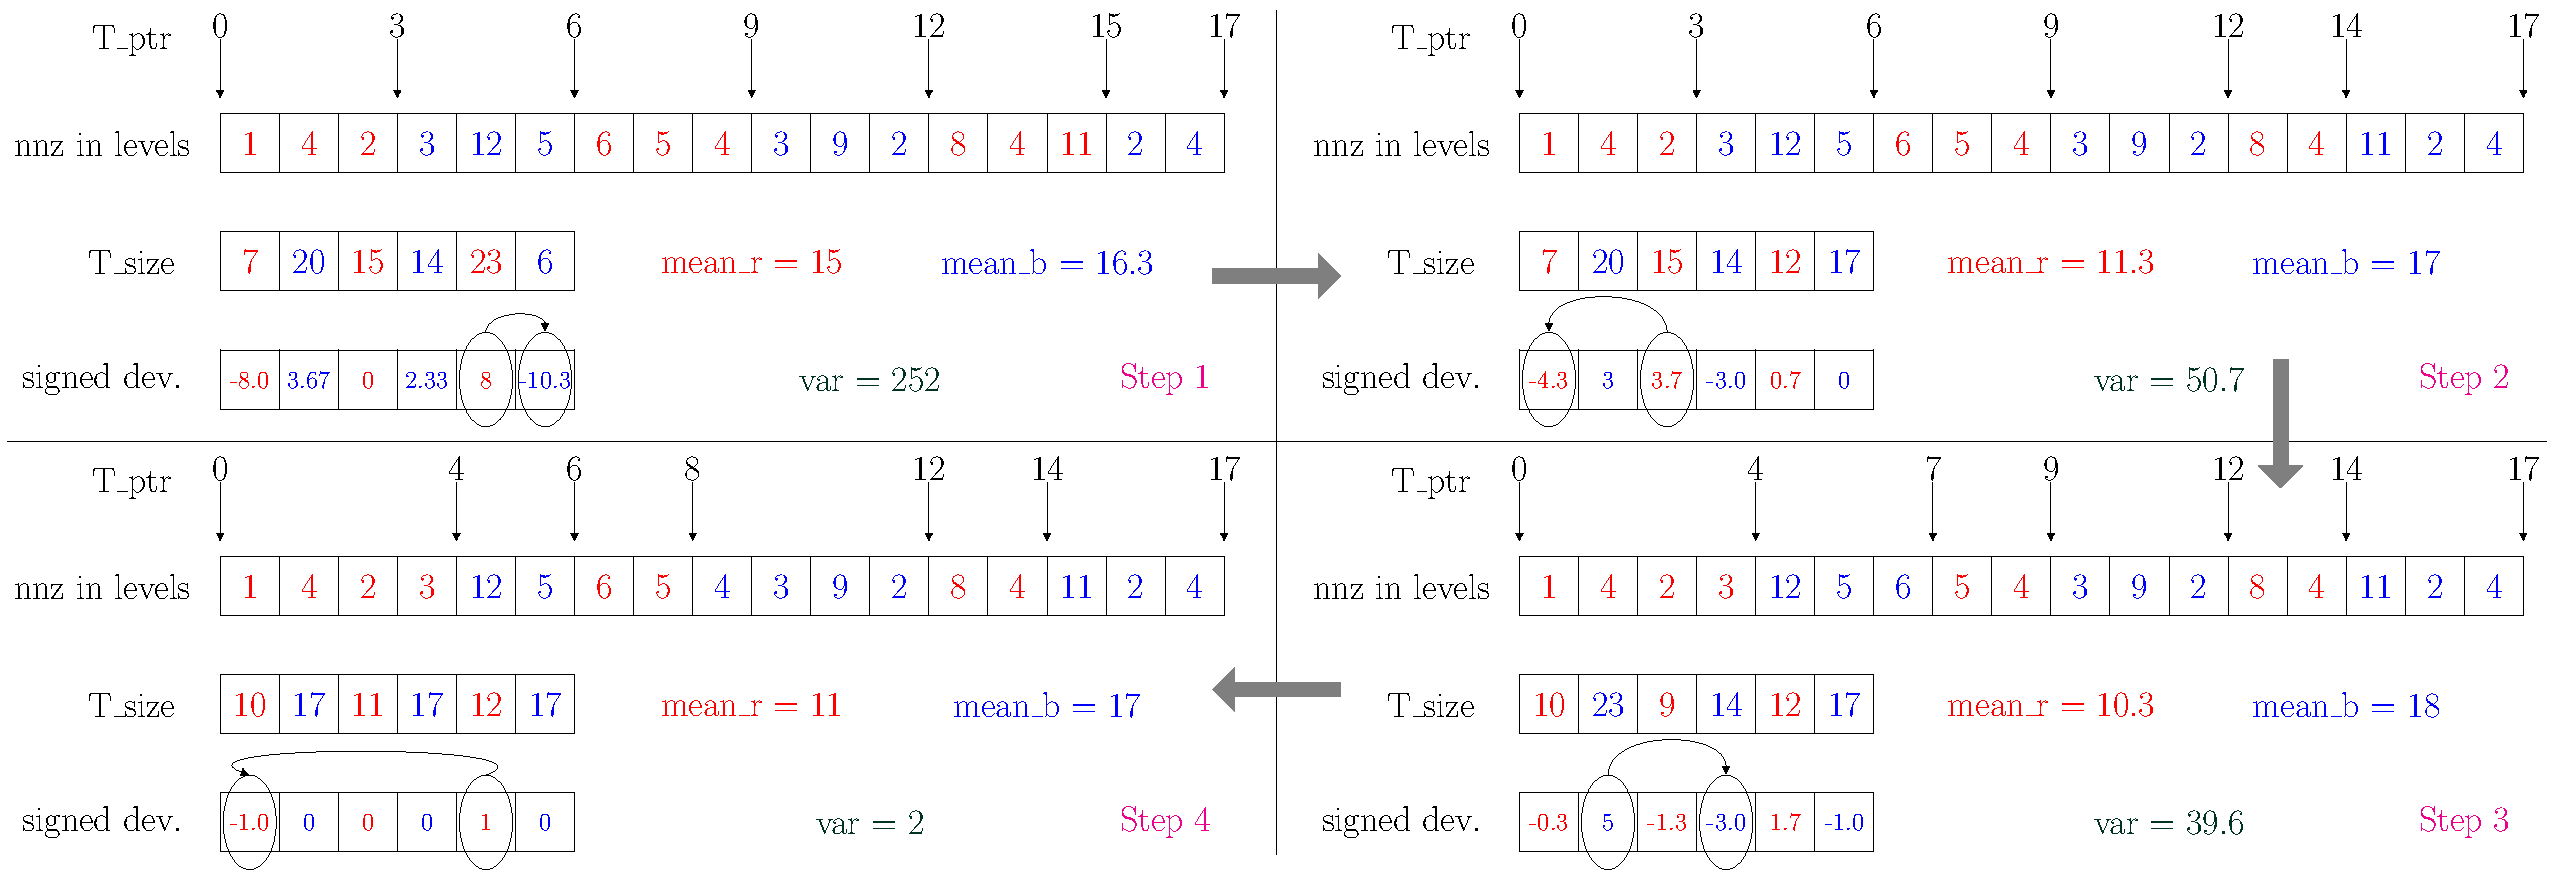
\includegraphics[height=0.22\textheight,width=\textwidth]{pics/load_balancing/lb_alg/lb_all}
   	\caption{Steps in load balancing (clockwise starting from top-left)}
   	\label{fig:lb_alg}
   \end{figure}
   
    
    \begin{figure}
      \begin{minipage}[c]{0.63\textwidth}
      	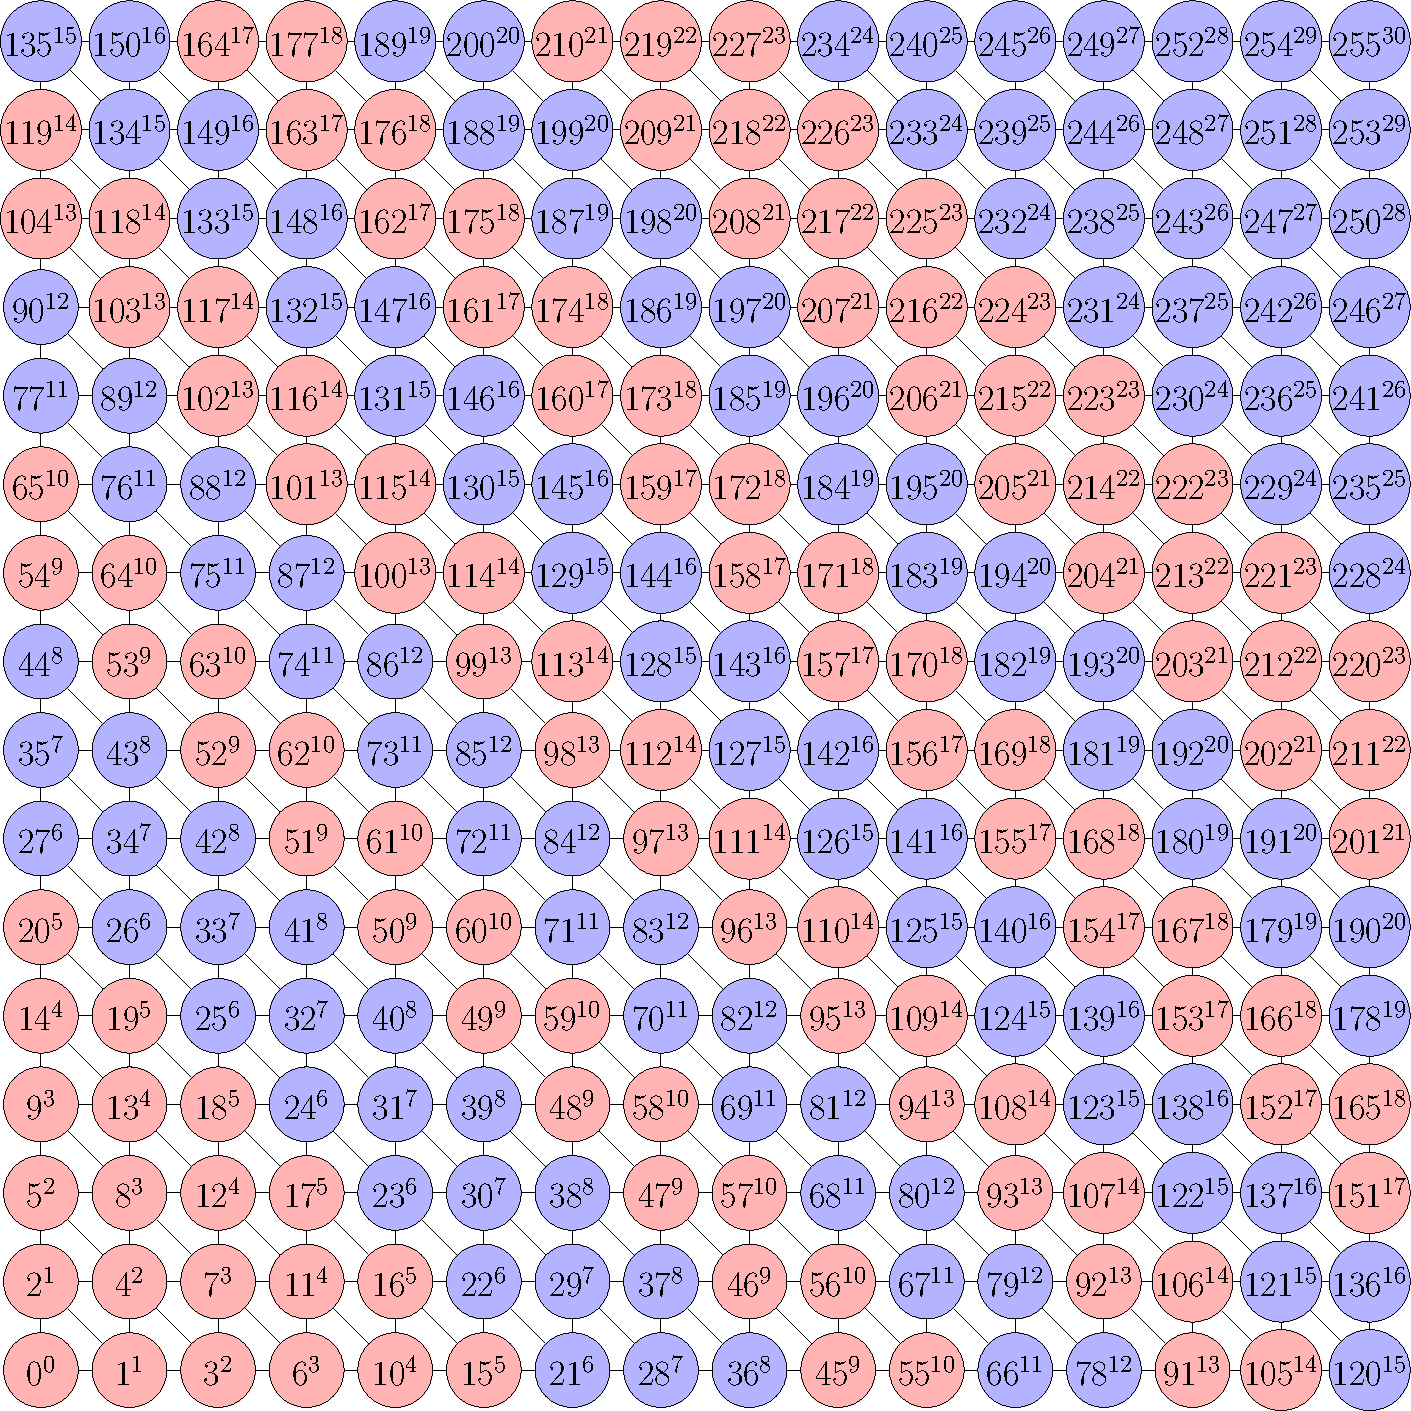
\includegraphics[height=0.26\textheight,width=0.9\textwidth]{pics/load_balancing/2d-7pt/stencil_2d_7pt}
      \end{minipage}\hfill
      \begin{minipage}[c]{0.34\textwidth}
      	\caption{After load balancing for five threads and \DTWO dependency on \STEX example, domain size $16 \times 16$. Note that \levelGroups at extreme end have more \levels due to less \nrows in each \level, while \levelGroups in middle having bigger \levels maintain two levels to preserve \DTWO constraint.
      	} \label{fig:2d_7pt_lb}
      \end{minipage}
     \end{figure}
     

	\subsection{Recursion}\label{subsec:REC}
	As seen above in \cref{subsec:DK} maximum amount of parallelism by the above approach depends on \totalLvl, also for most of the graphs as we approach the limit of parallelism there is not much room for load balancing, leading to imbalances. Depending on matrix and hardware underneath this might lead to inefficient utilization of resources. \Inorder to avoid this problem we use the concept of recursion and exploit further parallelism if required by the hardware. Idea here is to intelligently select sub-graph(s) of the entire matrix and apply all the four steps recursively on this \subgraph. In the following we will show this concept in the context of \DONE and  later we will extent it to \DK dependencies. Further we will discuss on the method employed to select proper sub-graph and to have a globally balanced load.
	
	\subsubsection{Distance-$1$}
	\LevelGroups which we constructed till now belongs to stage 1 of recursion and to make the explanations easier the stage number of recursion would be denoted as subscript \ie L$_s(i)$ denotes \level $i$ of stage $s$. Contrary to methods like \MCfull we didn't require each nodes in a color to be \DONE independent of each other rather we had a weak constraint as prescribed by \cref{corollary_dk}. Due to this there can exist more parallelism within a \levelGroup. For example in \cref{fig:rec_d1_s1} we see that within third \levelGroup (T$_1$(3)=L$_1$(3)) vertices $4 \not\xrightarrow{1} 5$ ($4$  \DONE independent to $5$), $4 \not\xrightarrow{1} 6$, $4 \not\xrightarrow{1} 7$ and $5 \not\xrightarrow{1} 7$, implying each of these pairs can be computed in parallel without any \DONE conflicts. This parallelism couldn't be exploited in stage 1 since vertices in $L_1(k)$ (here k=3) were connected to preceding \level $L_1(k-1)$ although some of them were not \DONE dependent within $L_1(k)$. \Inorder to exploit this parallelism we use the concept of recursion.
	
     \begin{figure}[thbp]
     	\centering
     	\subfloat[Example graph]{\label{fig:rec_d1_s1_a}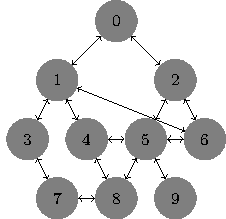
\includegraphics[width=0.26\textwidth, height=0.14\textheight]{pics/recursion/d1/rec_graph_s1/recursion_graph_1}}
     	\hspace{1.5em}
     	\subfloat[Stage 1 levels in graph]{\label{fig:rec_d1_s1_b}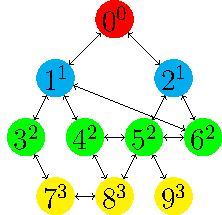
\includegraphics[width=0.26\textwidth, height=0.14\textheight]{pics/recursion/d1/rec_graph_s1/recursion_graph_2}}
     	\hspace{1.5em}
     	\subfloat[\DONE coloring]{\label{fig:rec_d1_s1_c}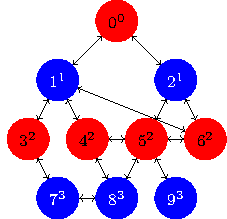
\includegraphics[width=0.26\textwidth, height=0.14\textheight]{pics/recursion/d1/rec_graph_s1/recursion_graph_3}}
        \caption{Shows potential for more parallelism. $T_1(2),T_1(3)$ and $T_1(4)$ has more parallelism.}
     	\label{fig:rec_d1_s1}
     \end{figure}
     
     Recursion begins by selection of a \subgraph of the matrix. A typical choice is a \subgraph induced by vertices in a \levelGroup of previous stage, more on the selection of \subgraph will be seen later in \cref{subsec:subgraph_selection}. For example let's choose \subgraph induced by $T_1(3)$ for recursion. The chosen \subgraph can be isolated from rest of the graph since  \DONE coloring step in stage 1 has already made \levelGroups in a sweep independent of each other. Now we just need to repeat all the four step explained previously (\cref{subsec:LEVEL_CONST} - \cref{subsec:LB}) to exploit parallelism within this \subgraph.
   
     \begin{figure}[thbp]
     	\centering
     	\subfloat[]{\label{fig:rec_d1_s2_a}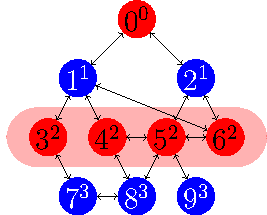
\includegraphics[width=0.26\textwidth, height=0.14\textheight]{pics/recursion/d1/rec_graph_s2/recursion_graph_stage2_1}}
     	\hspace{2.25em}
     	\subfloat[]{\label{fig:rec_d1_s2_b}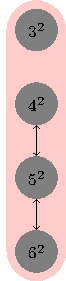
\includegraphics[width=0.08\textwidth, height=0.14\textheight]{pics/recursion/d1/rec_graph_s2/recursion_graph_stage2_2}}
     	\hspace{1.75em}
     	\subfloat[]{\label{fig:rec_d1_s2_c}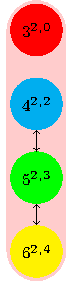
\includegraphics[width=0.07\textwidth, height=0.14\textheight]{pics/recursion/d1/rec_graph_s2/recursion_graph_stage2_3}}
     	\hspace{1.75em}
     	\subfloat[]{\label{fig:rec_d1_s2_d}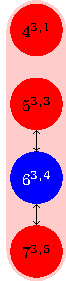
\includegraphics[width=0.07\textwidth, height=0.14\textheight]{pics/recursion/d1/rec_graph_s2/recursion_graph_stage2_4}}
	     \hspace{1.75em}
	     \subfloat[]{\label{fig:rec_d1_s2_e}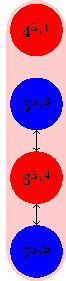
\includegraphics[width=0.07\textwidth, height=0.14\textheight]{pics/recursion/d1/rec_graph_s2/recursion_graph_stage2_5}}
     	\caption{Shows recursion being applied to $T_1(3)$. \Cref{fig:rec_d1_s2_b} shows the selected \subgraph, \cref{fig:rec_d1_s2_c} shows level construction step on the \subgraph, \cref{fig:rec_d1_s2_d,fig:rec_d1_s2_e} shows two possibility of \DONE coloring of the \subgraph}
     	
     	\label{fig:rec_d1_s2}
     \end{figure}
     
     \Cref{fig:rec_d1_s2} shows an illustration of applying stage 2 of recursion on $T_1(3)$ to find more parallelism. To incorporate the information of levels after recursion we extent the definition in \cref{eq:node_notation} to the following:
	 \begin{equation}
	    v^{i,j,k...} \implies v \in \set{L_1(i) \cap L_2(j) \cap L_3(k) \cap ...} 
	 \end{equation}
     
     Note that the \subgraphs might have multiple islands (group of vertices in a graph that are not connected to rest of the graph). For example vertex 4 in \cref{fig:rec_d1_s2_b} is an island in the considered \subgraph, similarly vertices 5,6,7 combine to form an island. Since an island is totally disconnected from the rest of the graph it can be executed in parallel to rest of the graph. To take advantage of this the starting node in next island is assigned with an increment of two levels, as seen in \cref{fig:rec_d1_s2_c}. Due to this there exists multiple valid \DONE configuration (here \cref{fig:rec_d1_s2_d,fig:rec_d1_s2_e}) and the selection of the optimal one will be done in the final load balancing step of a particular stage as described in \cref{subsec:LB}.    
     
     With this recursive process we were able to find independent \levelGroups ($T_{s+1}$) within \levelGroup of previous stage ($T_s$) and therefore the thread which works on $T_s$ has to spawn threads to parallelize within $T_{s+1}$.
     
	\subsubsection{Distance-$k$}
	For \DK the same procedure as \DONE applies, except with a slight difference in selecting the \subgraph. In \DONE we considered \subgraphs induced by \levelGroups, but for \DK coloring this is not sufficient. As seen in \cref{fig:rec_d2_wrong} for \DTWO coloring the selection of $T_1(2)$ as \subgraph did not guarantee \DTWO independency between \levelGroup $T_2$ within the \subgraph. This is due to the fact for $k>1$ dependency vertices $a,b$ within a \subgraph might be connected to a common vertex ($c$) outside the \subgraph leading to a \DK dependency between $a$ and $b$. In \cref{fig:rec_d2_wrong} we see 	$4 \xrightarrow{1} 2 \text{ \& } 7 \xrightarrow{1} 2 	\implies 4 \xrightarrow{2} 7$, but since vertex 2 was not in the \subgraph considered we missed this dependency. 

	
     \begin{figure}[thbp]
     	\centering
     	\subfloat[]{\label{fig:rec_d2_wrong_a}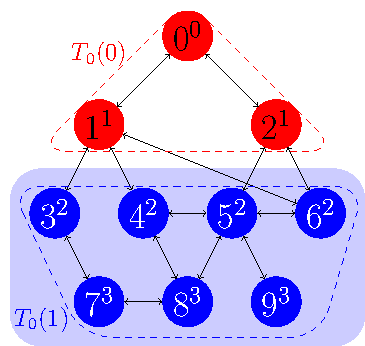
\includegraphics[width=0.23\textwidth, height=0.13\textheight]{pics/recursion/d2/wrong/recursion_graph_wrong_1}}
     	\hspace{0.6em}
     	\subfloat[]{\label{fig:rec_d2_wrong_b}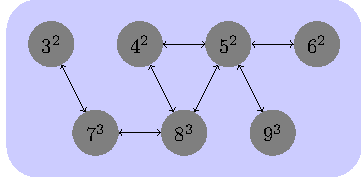
\includegraphics[width=0.23\textwidth, height=0.07\textheight]{pics/recursion/d2/wrong/recursion_graph_wrong_2}}
     	\hspace{0.6em}
     	\subfloat[]{\label{fig:rec_d2_wrong_c}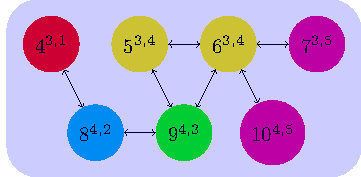
\includegraphics[width=0.23\textwidth, height=0.07\textheight]{pics/recursion/d2/wrong/recursion_graph_wrong_3}}
     	\hspace{0.6em}
     	\subfloat[]{\label{fig:rec_d2_wrong_d}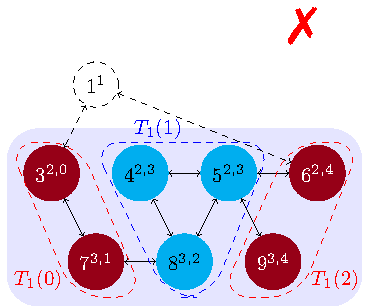
\includegraphics[width=0.23\textwidth, height=0.13\textheight]{pics/recursion/d2/wrong/recursion_graph_wrong_4}}
     	\caption{\Cref{fig:rec_d2_wrong_a,fig:rec_d2_wrong_b} shows \levelGroup induced \subgraph selected for recursion in case of \DTWO. But applying the four steps to this selected \subgraph does not guarantee a \DTWO independency between \levelGroup of same sweep (color) as seen in \cref{fig:rec_d2_wrong_d}}
     	\label{fig:rec_d2_wrong}
     \end{figure}
   
   \Inorder to resolve such dependency we have to consider an extra $(k-1)^{th}$ interface level(s) of the selected \subgraph for the level construction step. $k^{th}$ interface level of subgraph $L_s(j)$, denoted as $I^k(L_s(j))$, is defined as follows:
   \begin{equation*}
	   I^k(L_s(j)) = \set{u : u \xrightarrow{k} v \text{  } \forall v \in L_s(j) \text { and } u \notin L_s(j)}
   \end{equation*}
   For \DTWO this would mean we have to include 1 interface level, the new selection is illustrated in \cref{fig:rec_d2_correct}. With the new \subgraph selection for \DTWO coloring as seen in \cref{fig:rec_d2_correct_a}, the result after third step remains correct with respect to \DTWO coloring. In the example vertices 4 and 7 which had same color previously now gets a different color in (see \cref{fig:rec_d2_correct_d}). 
     
     \begin{figure}[thbp]
     	\centering
     	\subfloat[]{\label{fig:rec_d2_correct_a}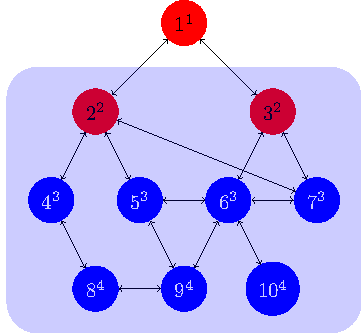
\includegraphics[width=0.22\textwidth, height=0.13\textheight]{pics/recursion/d2/correct/recursion_graph_correct_1}}
     	\hspace{0.6em}
     	\subfloat[]{\label{fig:rec_d2_correct_b}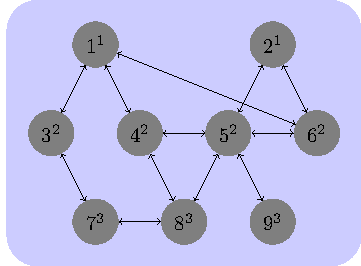
\includegraphics[width=0.22\textwidth, height=0.105\textheight]{pics/recursion/d2/correct/recursion_graph_correct_2}}
     	\hspace{0.6em}
     	\subfloat[]{\label{fig:rec_d2_correct_c}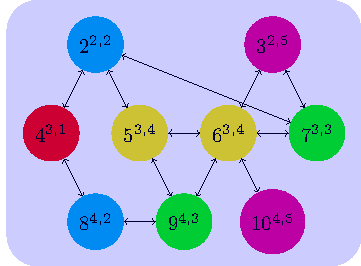
\includegraphics[width=0.22\textwidth, height=0.105\textheight]{pics/recursion/d2/correct/recursion_graph_correct_3}}
     	\hspace{0.6em}
     	\subfloat[]{\label{fig:rec_d2_correct_d}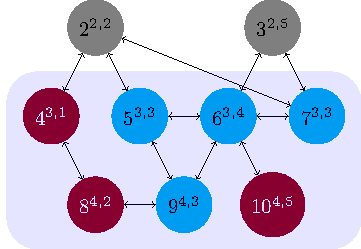
\includegraphics[width=0.22\textwidth, height=0.105\textheight]{pics/recursion/d2/correct/recursion_graph_correct_4}}
     	\hspace{0.6em}
     	\caption{Correct procedure of selecting \subgraph for \DTWO coloring. The \levelGroup $T_1(2)$ and it's $1^{st}$ interface level is chosen as the \subgraph as shown in \cref{fig:rec_d2_correct_a,fig:rec_d2_correct_b}. Level construction step is then applied to this \subgraph as seen in \cref{fig:rec_d2_correct_c}. Rest of the steps like permutation and \DK coloring is applied only to the \subgraph  chosen for recursion (here $T_1(2)$). Finally as seen in \cref{fig:rec_d2_correct_d} we get three \levelGroups at the end of recursion on $T_1(2)$.}
     	\label{fig:rec_d2_correct}
     \end{figure}
     
     Note that the interface levels have to be considered only in the first step namely level construction in the rest of the steps we just need to consider target \subgraphs induced by \levelGroups \ie in \cref{fig:rec_d2_correct} the \subgraph induced by $T_1(2)$. 
   
       \begin{figure}[H]
       	\begin{minipage}[c]{0.62\textwidth}
       		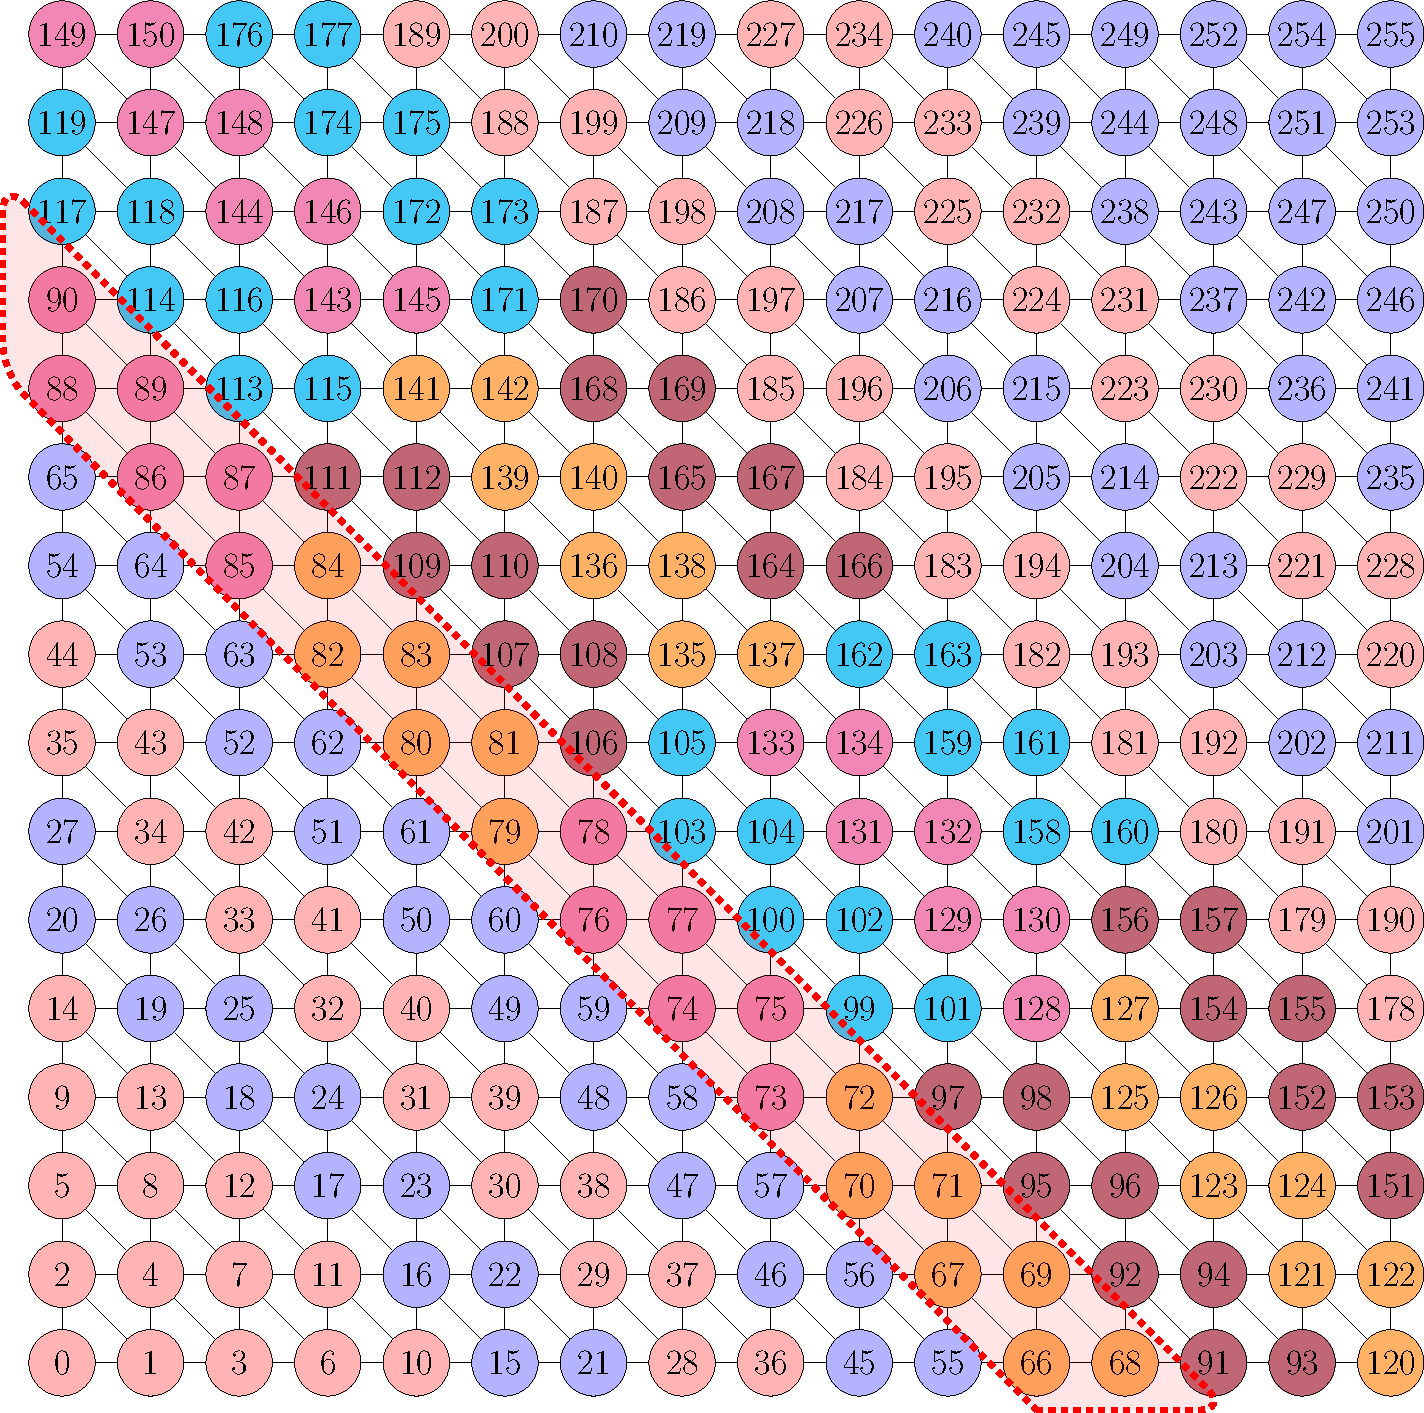
\includegraphics[height=0.25\textheight,width=0.9\textwidth]{pics/recursion/2d-7pt_example/2d-7pt/stencil_2d_7pt}
       	\end{minipage}\hfill
       	\begin{minipage}[c]{0.38\textwidth}
       		{\tt for parallel all \textcolor{red}{red}\\
       			\hspace*{1em} for parallel all \textcolor{amber}{orange}\\
       			\hspace*{1em} for parallel all \textcolor{magenta}{pink}\\
       		}
       		{\tt for parallel all \textcolor{blue}{blue}\\
       			\hspace*{1em} for parallel all \textcolor{carmine}{brown}\\
       			\hspace*{1em} for parallel all \textcolor{cyan}{cyan}\\
       		}
       		\caption{\STEX example for eight threads. Here recursion is applied on \levelGroups $T_1(5-8)$, to get more threads. The execution order of different \levelGroup is specified in the short code snippet on right. Note nested parallelism being used.}
       		\label{fig:rec_2d-7pt_graph}
       	\end{minipage}
       \end{figure}
     
     \Cref{fig:rec_2d-7pt_graph} (left) shows \DTWO coloring of \STEX example for eight threads. Here we see recursion is applied to \levelGroups $T_1(5),T_1(6),T_1(7)$ and $T_1(8)$. In this case each of the \levelGroups where recursion is applied spawns parallelism for two threads. The choice of \levelGroups to refine and number of threads needed from each recursion are determined using a global load balancing technique as will be explained in \cref{subsec:subgraph_selection}.
     
      \Cref{fig:rec_2d-7pt_graph} (right) shows the execution order of different \levelGroups. Note the usage of nested parallelism \ie for example thread responsible for $T_1(5)$ spawns two child threads to execute $T_2(1) \subset T_1(5)$ and $T_2(3) \subset T_1(5)$ in parallel, as well as $T_2(2) \subset T_1(5)$ and $T_2(4) \subset T_1(5)$ in parallel. At the end of each {\tt for parallel all color} there is synchronization between threads assigned to \levelGroup of corresponding color. Since each of the leaf need to synchronize only with it's siblings (leaves of same parent)  we use simple point to point synchronization scheme. 
          
       
	\subsubsection{Internal representation of recursively generated \boldmath{\levelGroups}} \label{subsec:level_tree}
	The recursive nature of our procedure allows to exploit more parallelism. However this introduces more complexity and one has to additionally respect the dependencies between stages and still observe the dependencies within one stage. The best idea is to have a data structure similar to the recursion, therefore we extent the \levelPtr data structure to a hierarchical tree data structure to store these informations. This data structure is called a \levelTree. The root of \levelTree contains information of entire domain, first child leaves of this root \ie leaves with depth 1 stores information about \levelGroups in stage 1 ($T_1(..)$), leaves with depth 2 stores information about \levelGroups in stage 2 ($T_2$) and so on. 
	
	 \begin{figure}[thbp]
		 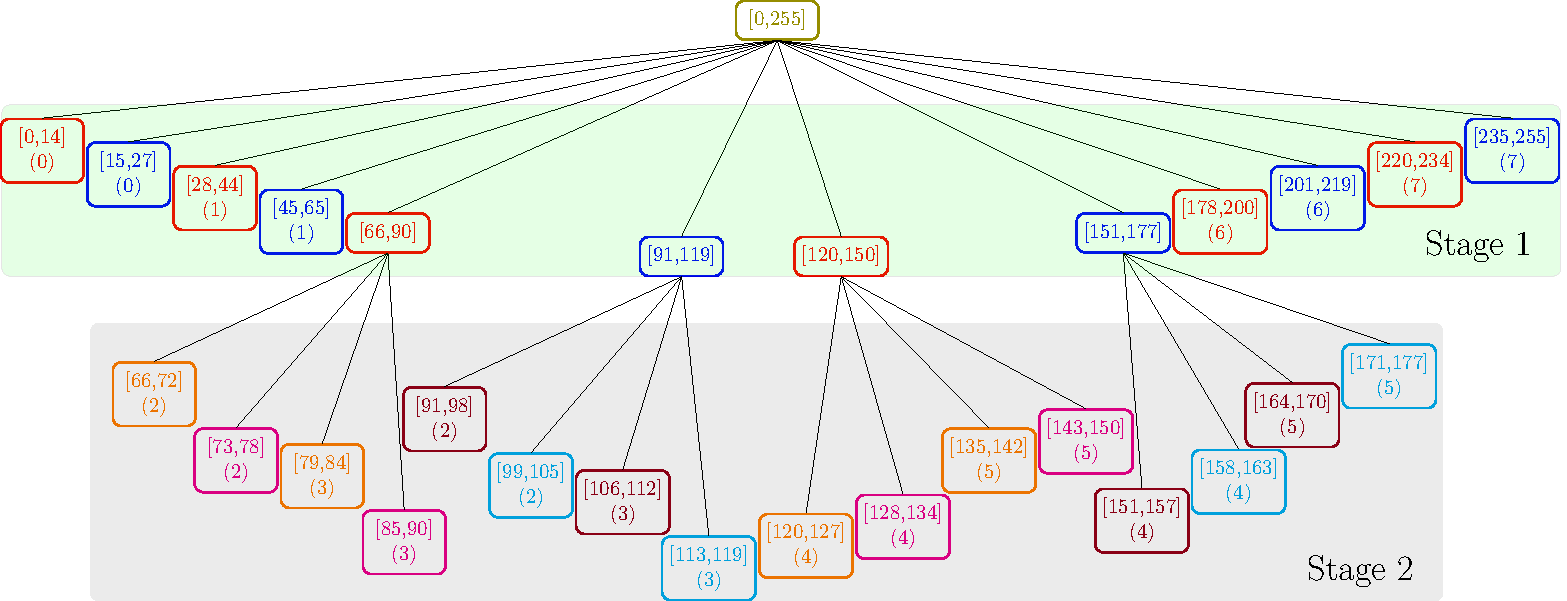
\includegraphics[width=\textwidth, height=0.2\textheight]{pics/recursion/2d-7pt_example/tree/tree}
	 	\caption{\levelTree corresponding to \STEX example for domain size $16 \times 16$, and 8 threads. The range (square brackets) specified in each leaves represent the vertices belonging to each \levelGroup, the number in bracket (parenthesis) represents the thread assigned to the \levelGroup in fill type pinning and the \nrowsEff (see \cref{Sec:param_study}) is represented within angle brackets.}
	 	\label{fig:rec_2d-7pt_tree}
	 \end{figure}

 
 \Cref{fig:rec_2d-7pt_tree} shows a \levelTree corresponding for \STEX example with 8 threads as seen in \cref{fig:rec_2d-7pt_graph}. The leaves in the tree that correspond to different \levelGroups and store various informations like the range of vertices or nodes that belong to this \levelGroup, the effective number of rows (\nrowsEff) that describes the quality which will be seen in \cref{Sec:param_study}, and other informations like threads assigned to specific \levelGroups.  Threads are assigned to each \levelGroup depending on the pinning strategy used. For example in \emph{fill} type pinning strategy one would pin thread 0 to $T_1(0)$ and $T_1(1)$, thread 1 to $T_1(2)$ and $T_1(3)$, thread 2 to $T_2(0)  \subset T_1(4)$, $T_2(1) \subset T_1(4)$, $T_2(0)  \subset T_1(5)$ and $T_2(1) \subset T_1(5)$, and so on as seen in \cref{fig:rec_2d-7pt_tree}. 
 
 Note that the \levelTree data structure is an exact replica of the nested parallelism being used as seen in \cref{fig:rec_2d-7pt_graph} (right). Therefore threads are spawned based on this \levelTree allowing for easy implementation of point to point synchronizations.

\subsubsection{Sub-graph selection and global load balancing} \label{subsec:subgraph_selection}
Parallelism required for hardware underneath can be obtained either by expanding the \levelTree horizontally \ie increasing \levelGroups within a stage or by expanding \levelTree vertically with the help of recursion. But as we have seen before in \cref{subsec:DK} the horizontal parallelism is limited and after a certain extent this would lead to load balancing. Similarly excessive usage of recursion is also not a good idea since data locality worsens due to local permutations within \subgraph. Therefore it is vital to find a proper balance and choose proper configuration. Furthermore just doing load balancing within a single stage is not the best, for example if we had equally balanced within stage 1 in \cref{fig:rec_2d-7pt_tree}, we would receive no benefit from recursion. Therefore a global load balancing becomes inevitable.

\Inorder to select proper \subgraph and do global load balancing we employ a simple algorithm to find proper weights for each \levelGroup ($T_s(i)$) in a particular stage, then depending on this weights, denoted as $w(T_s(i))$, we do load balancing with weights in the particular stage (as seen in \cref{alg:LB}, except weightage is given to \levelGroups). Finally if $w(T_s(i)) > 1$ we use recursion to achieve $w(T_s(i))$ parallel work in the next stage of $T_s(i)$. The basic structure of the algorithm employed to find weights is as follows:
\begin{enumerate}
	\item Find weights, $w(L_s(i))$ for each level in the current stage ($s$) by
		\begin{align*}
			w(L_s(i)) &= (\levelPtr_s[i+1] - \levelPtr_s[i])*\frac{\nthreadsMath}{\nrowsMath^{total}}\\
			\nthreadsMath &: \text{total parallelism required by hardware}\\
			\nrowsMath^{total} &: \text{number of vertices in graph}
		\end{align*}
	
	\item Starting from $w(L_s(0))$ sum up weights till they form a number ($a$) close to whole number ($b$). The closeness can be controlled by an efficiency parameter for stage $s$, $\epsilon_s$ is defined as:
	\begin{equation} \label{eq:epsilon}
		\epsilon_s =  1 - abs(a-b);
	\end{equation}
	All the \levels that are involved in the sum belongs to \levelGroups  operated by first thread in the current stage. The obtained number $b$ is chosen as weight for these \levelGroups \ie $w(T_s(0))=w(T_s(1))=b$. A local search is then done by increasing \levels in this \levelGroups to see if there is a better choice ($a$ close to $b$) with weight $b$, finally \levelGroups are formed with the best choice.  The weight for next \levelGroups are found by resetting the sum counter to zero and repeating the  procedure with \levels just after the current \levelGroups.
\end{enumerate}